\documentclass{article}

\usepackage[utf8]{inputenc}
\usepackage{longtable}
\usepackage{authblk}
\usepackage{adjustbox}
\usepackage{natbib}
\usepackage{graphicx}
\graphicspath{ {Imagenes/} }
\usepackage{array}
\usepackage{tabu}
\usepackage{multirow}
\usepackage{amsmath}
\usepackage{adjustbox}



\title{Indices de Desarrollo: Correlacion con la Poblaci<U+00F3>n Colombiana}
% autores
\renewcommand\Authand{, y }
\author[1]{\normalsize Juan Sebasti<U+00E1>n Cortazar}
\author[2]{\normalsize Mar<U+00ED>a Alejandra Restrepo}
\author[3]{\normalsize Juan Camilo Rueda}

\affil[1,2,3]{\small  Universidad de los Andes\\
\texttt{{js.cortazar533,ma.restrepot,jc.rueda169}@uniandes.edu.col}}



\date{29 de Junio de 2018}

%%%%

\usepackage{Sweave}
\begin{document}
\Sconcordance{concordance:Prueba2.tex:Prueba2.Rnw:%
1 33 1 1 0 63 1}


\maketitle


\begin{abstract}
En este trabajo se muestra el **Indice de Desarrollo Humano** (IDH) de Colombia por departamento. Donde a traves de estad<U+00ED>stica poblacional donde se mira el nivel de educaci<U+00F3>n, nivel de salud y ingresos per capita de los distintos departamentos para poder determinar los departamentos m<U+00E1>s vulnerables y los que tienen un mejor indice.Adicional se identifica una correlaci<U+00F3>n entre la poblaci<U+00F3>n y el IDH, por lo cual se hace una regresi<U+00F3>n entre el IDH y las poblaciones de cabecera por departamento y el total de poblaci<U+00F3>n de cada departamento con el IDH. 
\end{abstract}

\section*{Introducci<U+00F3>n}

El <U+00CD>ndice de Desarrollo Humano es una medida utilizada para determinar el crecimiento y el desarrollo de las zonas y los pa<U+00ED>ses teniendo no solo en cuenta el crecimiento econ<U+00F3>mico. Este <U+00ED>ndice busca medir no solo los PIB per c<U+00E1>pita de las personas, sino que busca entender el acceso a salud y a la educaci<U+00F3>n que determinan la posibilidad de crecimiento de las sociedades y sus capacidades de generar unas mejores condiciones de vida. 
El valor del IDH es la media geom<U+00E9>trica entre los <U+00ED>ndices normalizados de las tres dimensiones (Salud, Educaci<U+00F3>n y Nivel de Vida) como se muestra en la imagen \ref{IDH} a continuaci<U+00F3>n. 


%imagen de calculo del IDH
\begin{figure}[h]
\centering
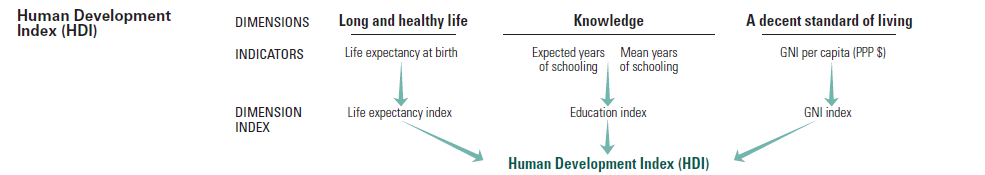
\includegraphics{hdiCalc}
\label {IDH}
\end{figure}

Para el c<U+00E1>lculo de cada uno de los <U+00ED>ndices se tienen unos limites inferiores y superiores que en conjunto con los valores del sector (ya sea pa<U+00ED>s o departamento) generan cada uno de los <U+00ED>ndices. En la tabla \ref{Tabla 1:}

%tabla boundary values

\begin{table}[h!]
\centering
  \begin{tabular}{l c c c}
  \hline
  Dimensiones & Indicador & Min & Max \\ [0.25ex]
  \hline \hline
  Salud & Expectancia de Vida (a<U+00F1>os) & 20 & 85 \\
  \multirow{2}{*}{Educaci<U+00F3>n} & Escolaridad Adultos & 0 & 18 \\ 
   & Esperanza educativa ni<U+00F1>os & 0 & 15 \\
  Nivel de Vida  & PIB per Capita (USD ctes 2011) & 100 & 75,000 \\
  \hline
  \end{tabular}
 \caption {Rango de Dimensiones IDH}
  \label{Tabla 1:}
\end {table}  

La variable Salud se genera a trav<U+00E9>s de un <U+00ED>ndice compuesto que refleja condiciones de salud en los hogares: protecci<U+00F3>n de salud, a trav<U+00E9>s del IGSS o de un seguro, n<U+00FA>mero de personas por dormitorio, tipo de acceso a agua y saneamiento y tipo de piso en la vivienda. Todos estos factores influencian la expectantica de vida y se calculan de la siguiente manera.

\[ Salud=\frac{LE-20} {85-20} \]

Donde $LE = Expectativa de Vida$
La variable Educaci<U+00F3>n es un indicador compuesto que incluye la escolaridad alcanzada por adultos mayores de 25 a<U+00F1>os y la esperanza educativa en ni<U+00F1>os. En el primer indicador se mide la tasa de alfabetizaci<U+00F3>n de adultos en el segundo se mide la tasa bruta combinada de matriculaci<U+00F3>n en educaci<U+00F3>n primara, secundario y superior, as<U+00ED> como los a<U+00F1>os de duraci<U+00F3>n de la educaci<U+00F3>n obligatoria. El c<U+00E1>lculo del <U+00ED>ndice de educaci<U+00F3>n se define de la siguiente manera
\[Educaci<U+00F3>n= \frac{EA + EN} {2} \]
Donde
\[EA= \frac{Prom de a<U+00F1>os de educaci<U+00F3>n adultos} {18}  \]
\[EN= \frac{Prom de a<U+00F1>os de educaci<U+00F3>n ni<U+00F1>os} {15}  \]

La variable del nivel de vida mide el PIB per c<U+00E1>pita de una zona o pa<U+00ED>s teniendo en cuenta un m<U+00ED>nimo esperado y un m<U+00E1>ximo. La formula es la siguiente

\[Nivel de Vida = \frac {Ln(PIBx)<U+2013>Ln(100)} {Ln(75,000)-Ln(100)} \]






\end{document}
